\subsection{Electromagnetic Calorimeter} 
\label{sec:ecal}

The Ecal, depicted in Fig. \ref{fig:ecal}, consists of 442 lead-tungstate PbWO$_4$ crystals with avalanche photodiode (APD) readout and amplifiers. Those have all similarly short pulse widths, so that they can run at very high rates. Indeed, the expected high radiation and high rate environment, together with a high magnetic field in close proximity, essentially imposed lead-tungstate (PbWO$_4$) crystals with APD readout. The lead tungsten (PbWO$_4$) crystals will be taken from the IC of the JLab CLAS detector, which was originally build in IPN Orsay and run for 10 years with success. Crystals in the ECal are arranged in two modules. There are 5 layers in each module; four layers have 46 crystals and one has 37. The ECal is mounted downstream of the analyzing dipole magnet at the distance of about 148 cm from the upstream edge of the magnet. The two ECal modules are positioned just above and below a vacuum chamber, through which the beam and the “wall of flame” pass in vacuum. At its closest point, the edge of the crystal is at 3.7 cm from the beam. In order to maintain stable performance of the PbWO$_4$ calorimeter, the crystals and APDs are enclosed within a temperature stabilized environment, held constant at the level of 1\!\char23F. The expected energy resolution of the system from operational experience with the IC (“inner calorimeter”), an Inner Calorimeter which had been used in the CLAS experiment and built by the IPN Orsay group, is $\sigma_E/E \sim 4.5\%/\sqrt{E}$ (GeV). As in the IC, PbWO$_4$ modules are connected to a motherboard that provides power and transmits signals from individual APDs and pre-amplifier boards. The ECal data is digitized in the JLAB FADC250, a 250 MHz flash ADC developed for the 12 GeV Upgrade detectors. The full analogue information from the FADCs coupled with the fine spatial information of the calorimeter and is available to the trigger, which uses energy deposition, position, timing, and energy-position in correlations to reduce the trigger rate to a manageable 30 kHz (see section \ref{seq:ECalTrigger} for details).

\begin{figure*}[t]
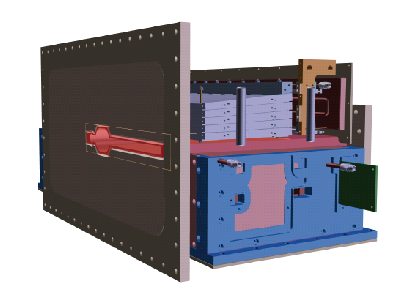
\includegraphics[scale=0.7]{ecal/ECal.png}
\caption{\small{Cut-away view of the Ecal, showing the vacuum flange which mates to the magnet vacuum chamber on the left, holes for the electron beam and the “wall of flame” in the Ecal vacuum chamber (in red), crystal positions in the upper module, and the temperature control box in blue in the lower module.}}\label{fig:ecal}
\end{figure*}

The role of the electromagnetic calorimeter in the HPS experiment is two folds, the ECal is the main trigger for the data acquisition and it should, at the same time, allow for good electron identification. Indeed, the trigger algorithm is based on energy and position measurements, and requires very short time coincidence in order to suppress orders of magnitude higher background. The calorimeter DAQ system will be based on flash ADCs and trigger modules developed for JLAB 12 GeV upgrade.

For a discovery experiment like HPS, where backgrounds need to be strongly suppressed but also well understood, the trigger can be an important source of experimental bias. Therefore, it needs to be very well controlled. In particular, having a stable and known threshold is necessary in order to avoid a bias in the event selection at the trigger level. This uniformity and stability can be achieved with the installation of a on-line gain monitoring system. This system will consist on the introduction of light in the front of the crystals with optic fibers to test the APDs response. It will therefore be sensitive to both transparency losses of the crystal and gain variations from the APDs. Such a system has been developed for several experiments (CMS at CERN for instance) with various light sources. The system will be developed in IPN Orsay in 2013 and in the first half of 2014, before being shipped and installed in Virginia for the commissioning run at the end of 2014. We choose, for their low cost, to use two different mono color LEDs as light sources, to monitor the gain variations. A blue light, which corresponds to the domain of emission in the crystals, is very sensitive to the presence of color centers, produced by radiation damage. This light source is very useful to test variations of the gain in the main domain of emission used for detection and since impurities can anneal at room temperature, such monitoring can be sensitive to increasing gain output too, when the radiation exposure is reduced for a long period of time. A red colored light, less sensitive to the color centers, permits monitoring the APD gains more directly and thereby separate effects of APD and electronics from crystal transparency and provide clear information on the state of the electronics and crystals. The main challenge for the system is to guarantee stability at a level better than a percent to be able to identify and to adapt to the transparency variations. The test of the system will be carried on at IPN Orsay, in order to guarantee this efficiency and also to test radiation resistance of the various materials.

The second major improvement to be done for the calorimeter consists in the implementation of new APDs, by replacing old 5x5 mm2 APDs with 10x10 mm2, Hamamatsu S8664-1010. The renewal of the APDs will resolve both major issues with present modules of HPS calorimeter. First, new APDs from Hamamatsu have much better performance than the ones which are now installed on lead-tungstate crystals. Data from Hamamatsu shows that APDs made from the same wafer have excellent uniformity. With +/- 10\% known uniformity at the gain of 100, variations in bias voltage are ~4.5 V. Moreover, data provided for samples of 1300 the bias voltage difference is ~50 V, when for APDs now we have (442 pieces) the voltage difference is more than 100V. So, it is clear that with new APDs the main issue of uniform response of the calorimeter in the trigger can be achieved. Second, 4 times larger readout area will ensure 4 times more light collection and therefore 4 time larger signal from APDs. This will allow the use of different amplifier modules with lower gain that in turn will decrease electronic noise. Tests performed for another calorimeter, now in production for JLAB Hall-B, showed that the same type of amplifier boards with factor 2 lower gains have noise level on the order of 5 MeV. New amplifiers have therefore to be designed to fit these new conditions and optimize the higher signal; these will be designed by IPN Orsay engineers in connection with the HPS team. Then, the lower noise will allow to lower the acquisition thresholds and to improve the energy resolution, but it will also open the possibility to calibrate the modules with cosmic muons, while they are installed in the detector. Minimum ionizing energy deposition in PbWO$_4$ crystals of HPS calorimeter from cosmic muons passing through perpendicular to the crystal axis is of ~15 MeV. If energy thresholds can be moved close to 5~MeV, then MIP peak will be seen and calorimeter can be calibrated and monitored with cosmic muons.

